\chapter*{Background}
\addcontentsline{toc}{chapter}{Background}
\section{Literature Review}
In order to understand the design requirements of the library, a literature review needed to be performed. The scope was
narrowed down to 3 systems that showed promise and were broadly representative of the antenna configuration that future
systems would adopt. Most systems will adopt one of the following setups
\begin{enumerate}
    \item Monostatic
    \item Leveled Multistatic
    \item Fully Multistatic
\end{enumerate}
\noindent These terms relate to the position of antennas around the breast tissue and how the resulting scan data would
be structured. \hfill \break

\subsection{MARIA M4}
The first system we will look at is the MARIA M4 system developed by Preece et al within the Electrical and Engineering
Department of the University of Bristol \cite{preeceMARIAM4Clinical2016}. This is the 4th iteration in a series of MARIA systems that evolved from a
system of 16 UWB antennas to 60 antennas in the current system. These all operate in a multistatic configuration,
meaning that any antenna in the array can listen to any other antenna in the array, an example of which can be seen in
Figure \ref{fig:MultistaticExample}. This figure shows a top-down view, however, one can imagine this being generalized
to a hemisphere of antennas around the breast. \hfill

\begin{figure}
    
\includegraphics[width=0.3\textwidth]{multistaic.png}
    \centering
    \caption{Example of a Fully Multistatic Configuration (Top-Down)}
    \label{fig:MultistaticExample}
\end{figure}

\noindent As stated before, the MARIA M4 systems makes use of the UWB spectrum over a frequency range of 3.0 to 8.0 GHz. A
VNA was used to step through the frequencies and collect the scans from the antenna. The system exploits the inherent
symmetry in the antenna reciprocity to halve the number of channels (made of a transmitting and receiving antenna)
collected, thereby speeding up the scan time. For the MARIA M4 system, this equates to a 1770 reduction in the number of
channels collected. Figure \ref{fig:MARIAM4}, shows the antenna array used in the M4 system (a), as well as the M5
system (c) which is an integrated package.


\begin{figure}
    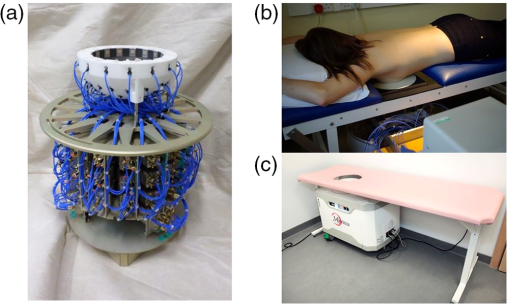
\includegraphics[width=0.5\textwidth]{MARIA_M4.png}
    \centering
    \caption{The MARIA M4 and M5 system. (a) The MARIA M4 antenna array. (b) The M4 in a clinical setting. (c) The integrated M5 package \cite{preeceMARIAM4Clinical2016}}
    \label{fig:MARIAM4}
\end{figure}

\noindent The team scanned 86 participants, with a mean age of 51.4 and a range of 24 - 78 years old. The M4 system showed a sensitivity of
74\% (64/86) when compared with the "gold-standard' of an ultrasound. The "sensitivity" was determined based on the
ability of the M4 system to localize a lesion as it correlated with the location in the ultrasound image. The research
team also divided the group into pre-/peri- and post- menopausal women and found that the sensitivity was 75\% and 73\%
respectively. However, the reliability of these results are called into question when considering the sample size of the
study. Given a sample size of 86, and assuming a normal distribution and that the results are statistically significant
($p < 0.05$, Z = 1.96), a 10.58\% margin of error was calculated. While this may not be enough to conclusively prove
that the M4 system is a viable alternative to Mammograms, it is enough to show promise. With a larger sample size, this
margin of error could be narrowed further.

\subsection{Wavelia}
The second system that was considered was the Wavelia Microwave Breast Imaging System developed by MVG Industries
\cite{moloneyWaveliaMicrowaveBreast2021}. The Wavelia system integrates the imaging system as well as the examination
bed into one complete package (Figure \ref{fig:WaveliaSystem}). The integrated package makes the Wavelia system an
appealing choice for some hospitals, however, its large size may be a barrier to adoption in some facilities where space
is a premium. \hfill \break

\begin{figure}
    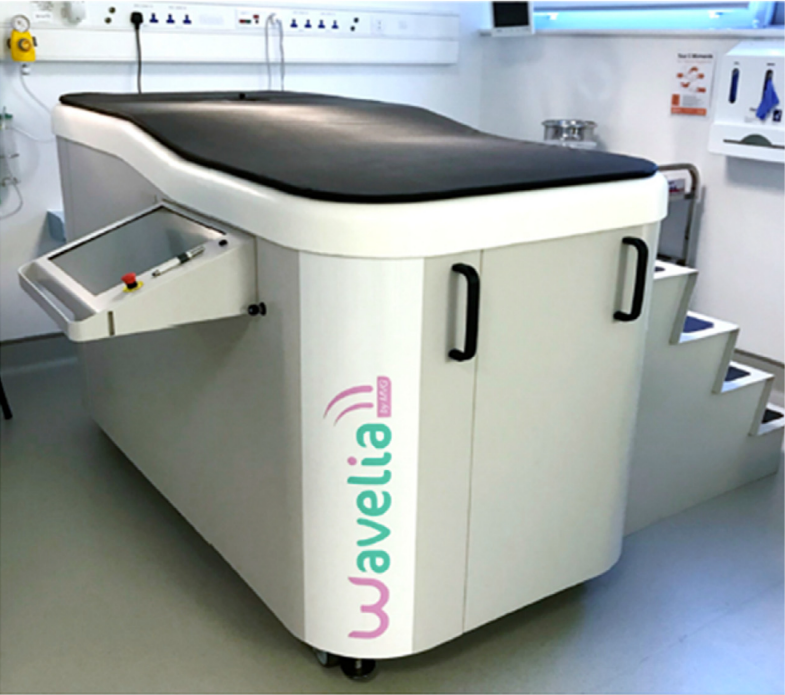
\includegraphics[width=0.5\textwidth]{Wavelia.png}
    \centering
    \caption{The Wavelia System \cite{moloneyWaveliaMicrowaveBreast2021}}
    \label{fig:WaveliaSystem}
\end{figure}

Like in the MARIA M4 system, patients lie in a prone position and place their breasts in the circular cutouts on the
bed. The system then begins to create a 3D reconstruction of the exterior of the breast using a stereoscopic camera.
This also allows for the breast volume to be explicitly calculated rather than being inferred like in the MARIA system.
The Wavelia makes use of the UWB spectrum when imaging the breast, although they opt for a narrower frequency range of
0.5 - 4.0 GHz compared to the 3.0 - 8.0 GHz range of the MARIA system. The antenna configuration, unlike the MARIA system, is an array of 18 Vivaldi-type probes arranged in a concyclic manner
on a horizontal plane. These antennas operate in a Multistatic manner and image the breast in sections parallel to the
coronal plane. The entire antenna assembly moves downwards in 5mm intervals to image the entire breast (Figure \ref{fig:LeveledMultistaticExample}). This is a
leveled multistatic system as opposed to the fully multistatic system in the MARIA M4. This leveled multistatic approach
has the benefit of a theoretically infinite vertical resolution. If the radiologist wanted a finer resolution along the
coronal plane, they would just have to tweak the array vertical step size, rather than having to manufacture an entirely
new antenna array, like in the MERIT system. This leveled approach also allows the parameters of the reconstruction
algorithm to be easily changed based on the particular section of the breast that we are imaging. The fully multistatic
approach, however, would need significant additional logic in the post-processing steps to determine which channels are
coplanar with a particular section. \hfill \break

\begin{figure}
    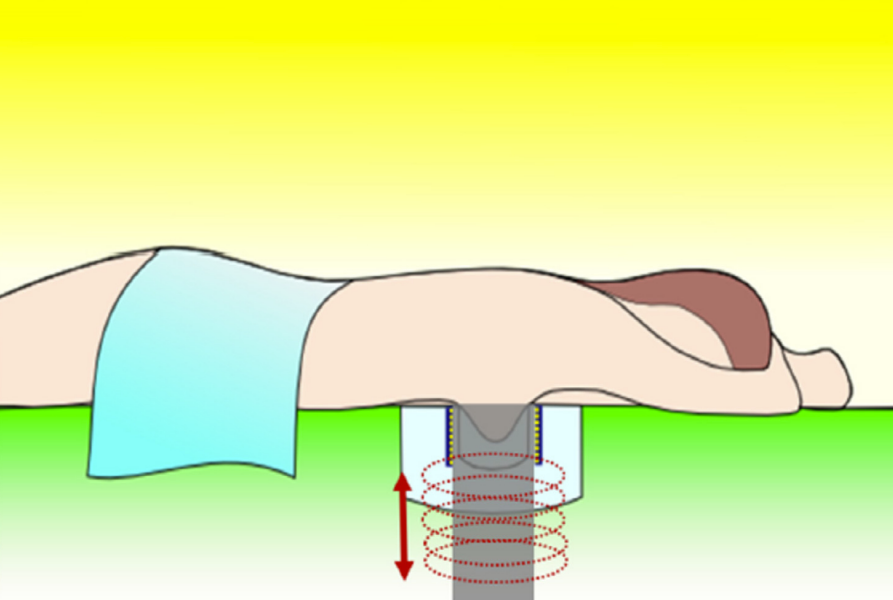
\includegraphics[width=0.5\textwidth]{LeveledMultistatic.png}
    \centering
    \caption{The Leveled Multistatic Approach of Wavelia \cite{moloneyWaveliaMicrowaveBreast2021}}
    \label{fig:LeveledMultistaticExample}
\end{figure}

\noindent The Wavelia paper \cite{moloneyWaveliaMicrowaveBreast2021} conducted a feasibility study on 25 female
participants. While the results aren't statistically significant, they do demonstrate the strengths of the Wavelia
system. 11 of the participants had a biopsy confirmed carcinoma and out of these, the Walia system detected 9 lesions,
with 7 being located to the appropriate region. Overall the system detected an abnormality in 21 of the 24 participants,
leading to a sensitivity of 87.5\%. The researchers do note some limitations of the Walia system, namely it can't detect
any lesions smaller than 10mm. This is significant since the size of the detected lesion plays a big factor when
deciding whether a lesion is cancerous or not. Another limitation of the system is that breast sizes that are too small
cannot be scanned in any great detail by the Wavelia system. Due to the patients being in the prone position, their
breast tissue needs to hang down far enough to have multiple sections of their breast be imaged by the antenna array.
The researchers are working on a subsequent system that should address all the aforementioned limitations. Overall the
participants had a positive outlook on the system. 23 out of the 25 women said that they would recommend the procedure
to other women and all of the women agreed that the information provided was clear and well understood.

\subsection{TSAR}